
In this analysis, the charged Higgs boson is decaying to the $c$ and $\bar{s}$ 
quark. The invariant mass of the $c\bar{s}$ system (\mjj) is thus used as the 
final observable. The \mjj distribution of two highest \pt, non-b-jets is
shown in Figure~\ref{subfig:mjj_muBTag} and \ref{subfig:mjj_eleBTag} for
both channels. For the true semileptonic \ttbar events, the mean of the \mjj 
should be close to 80.0 GeV, which is the mass of the W Boson. However, the mean of
\mjj, as shown in Figure~\ref{subfig:mjj_muBTag} and (\ref{subfig:mjj_eleBTag}),
is about 138 GeV because the two light jets in every event may not necessarily 
come from the decay of a W Boson. Secondly, the \mjj distribution has a long tail 
which might constrain the search for new resonances in the dijet mode. 
\begin{figure}
    \centering
    \subfigure[\mjj with reco jets after b-jet selection \label{subfig:mjj_muBTag}]
    {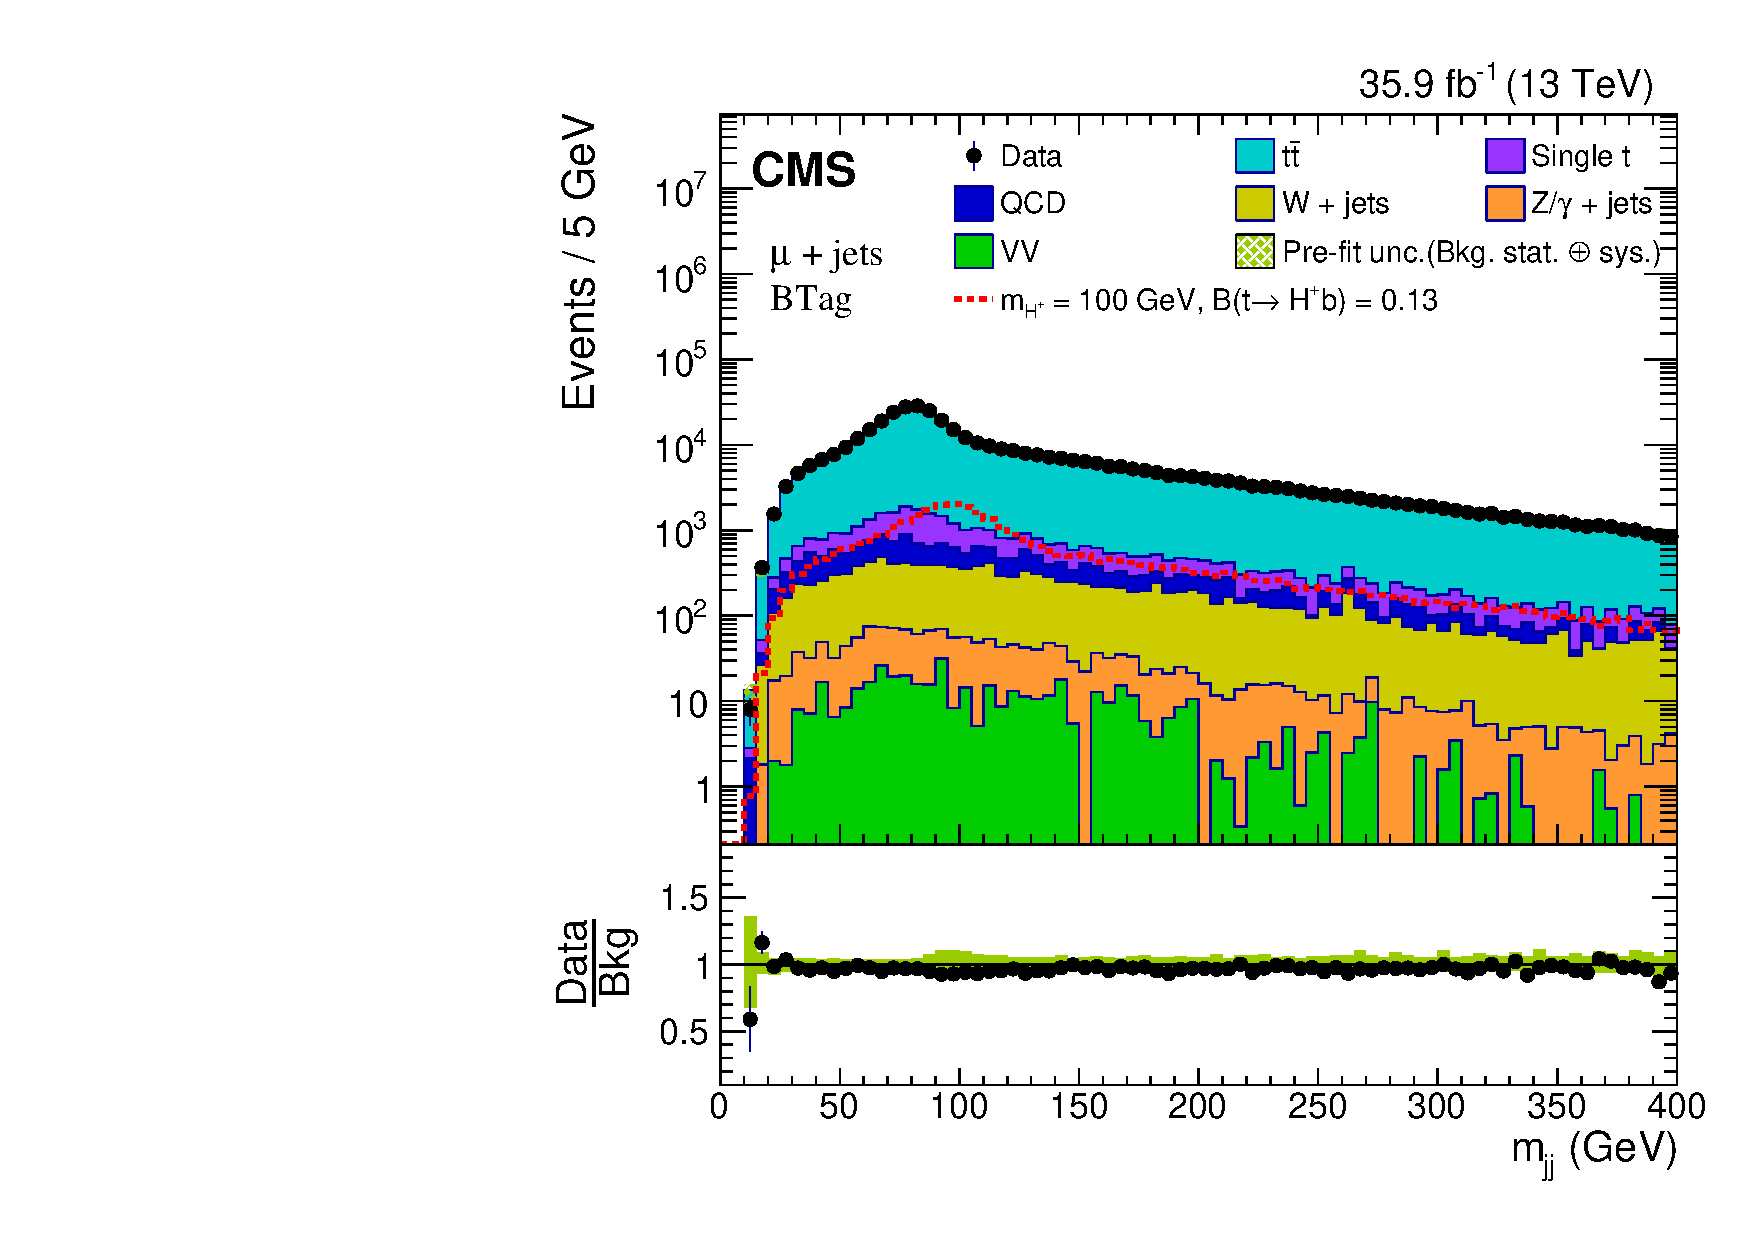
\includegraphics[width=0.49\linewidth]{Image/Muon/BTag/mjj_muBTag.pdf}}
    \subfigure[\mjj with reco jets after b-jet selection \label{subfig:mjj_eleBTag}]
    {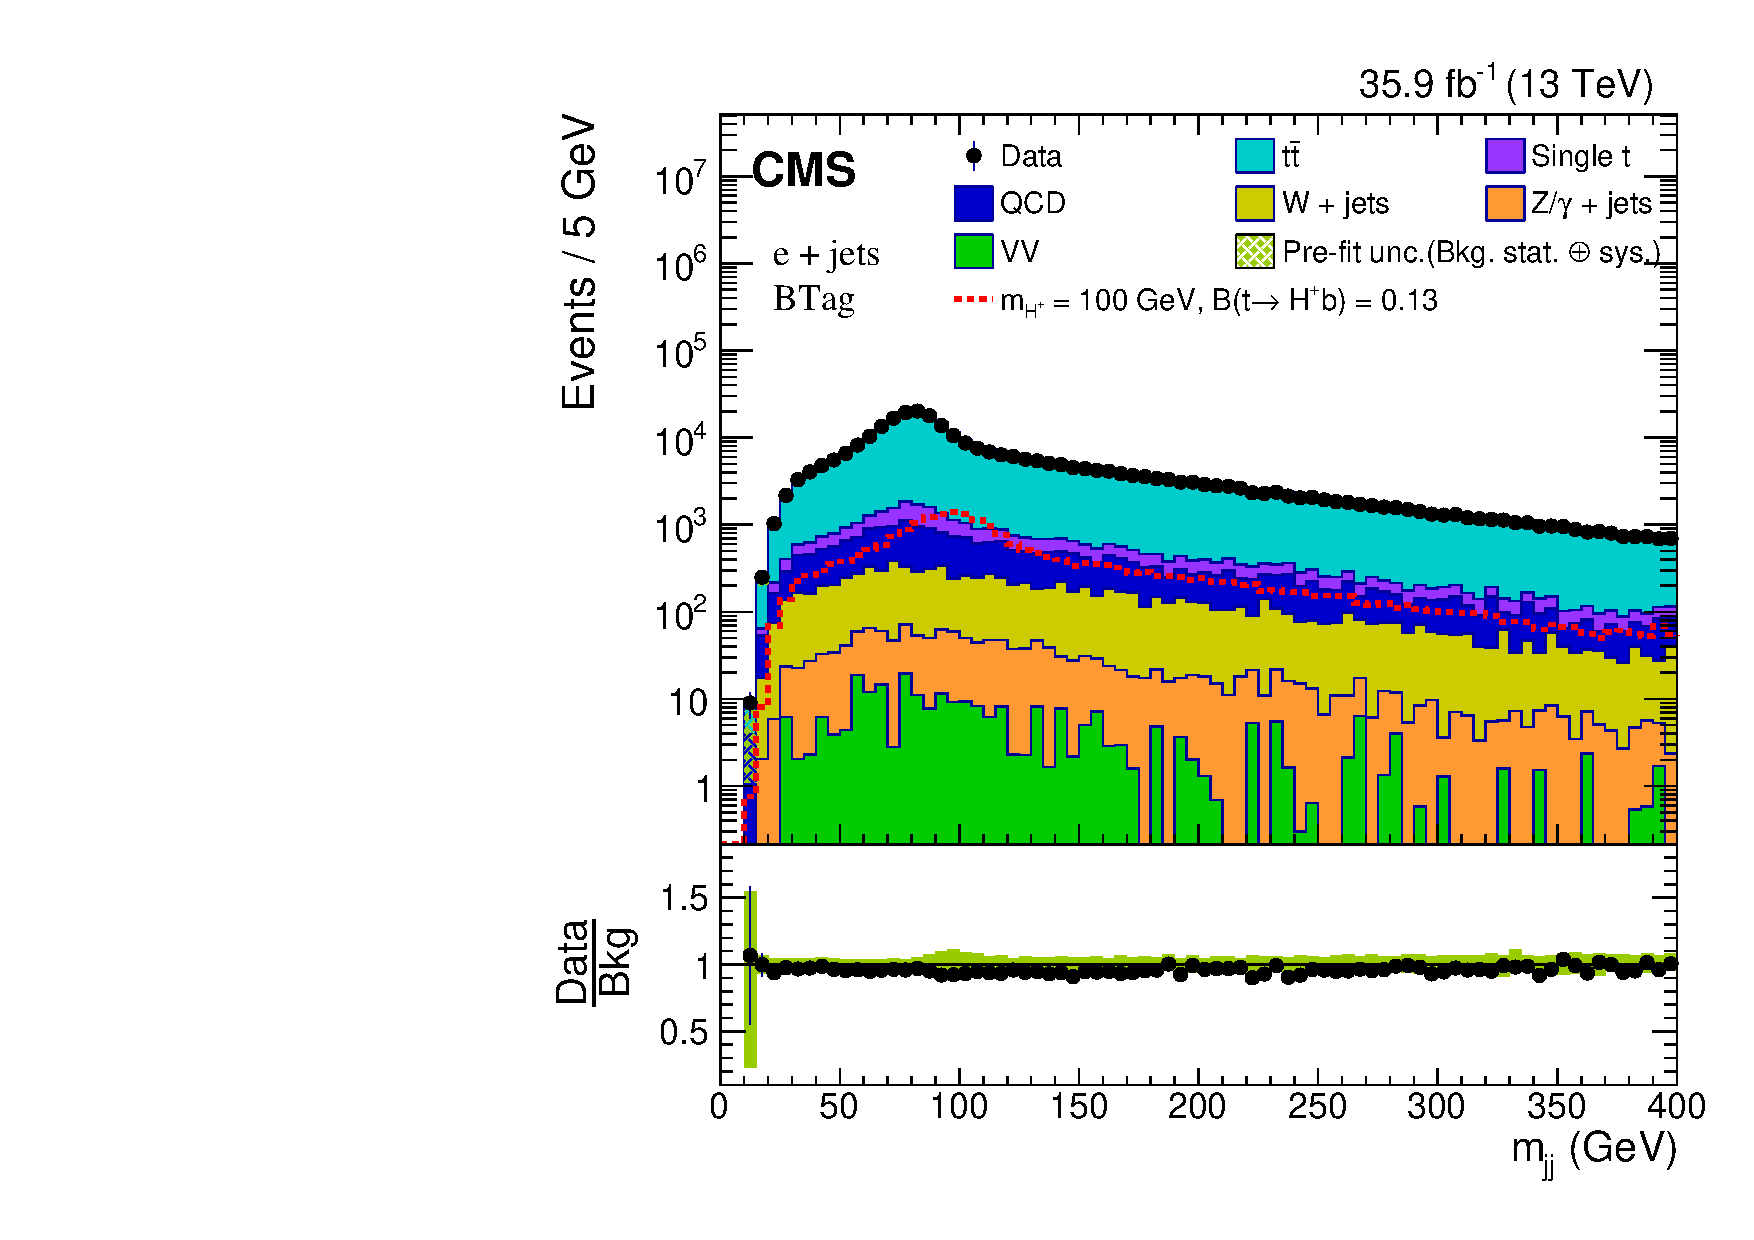
\includegraphics[width=0.49\linewidth]{Image/Electron/BTag/mjj_eleBTag.pdf}}
    \vfil
    \subfigure[\mjj with kinematic fitted jets after KinFit selection \label{subfig:mjj_kfit_muKinFit}]
    {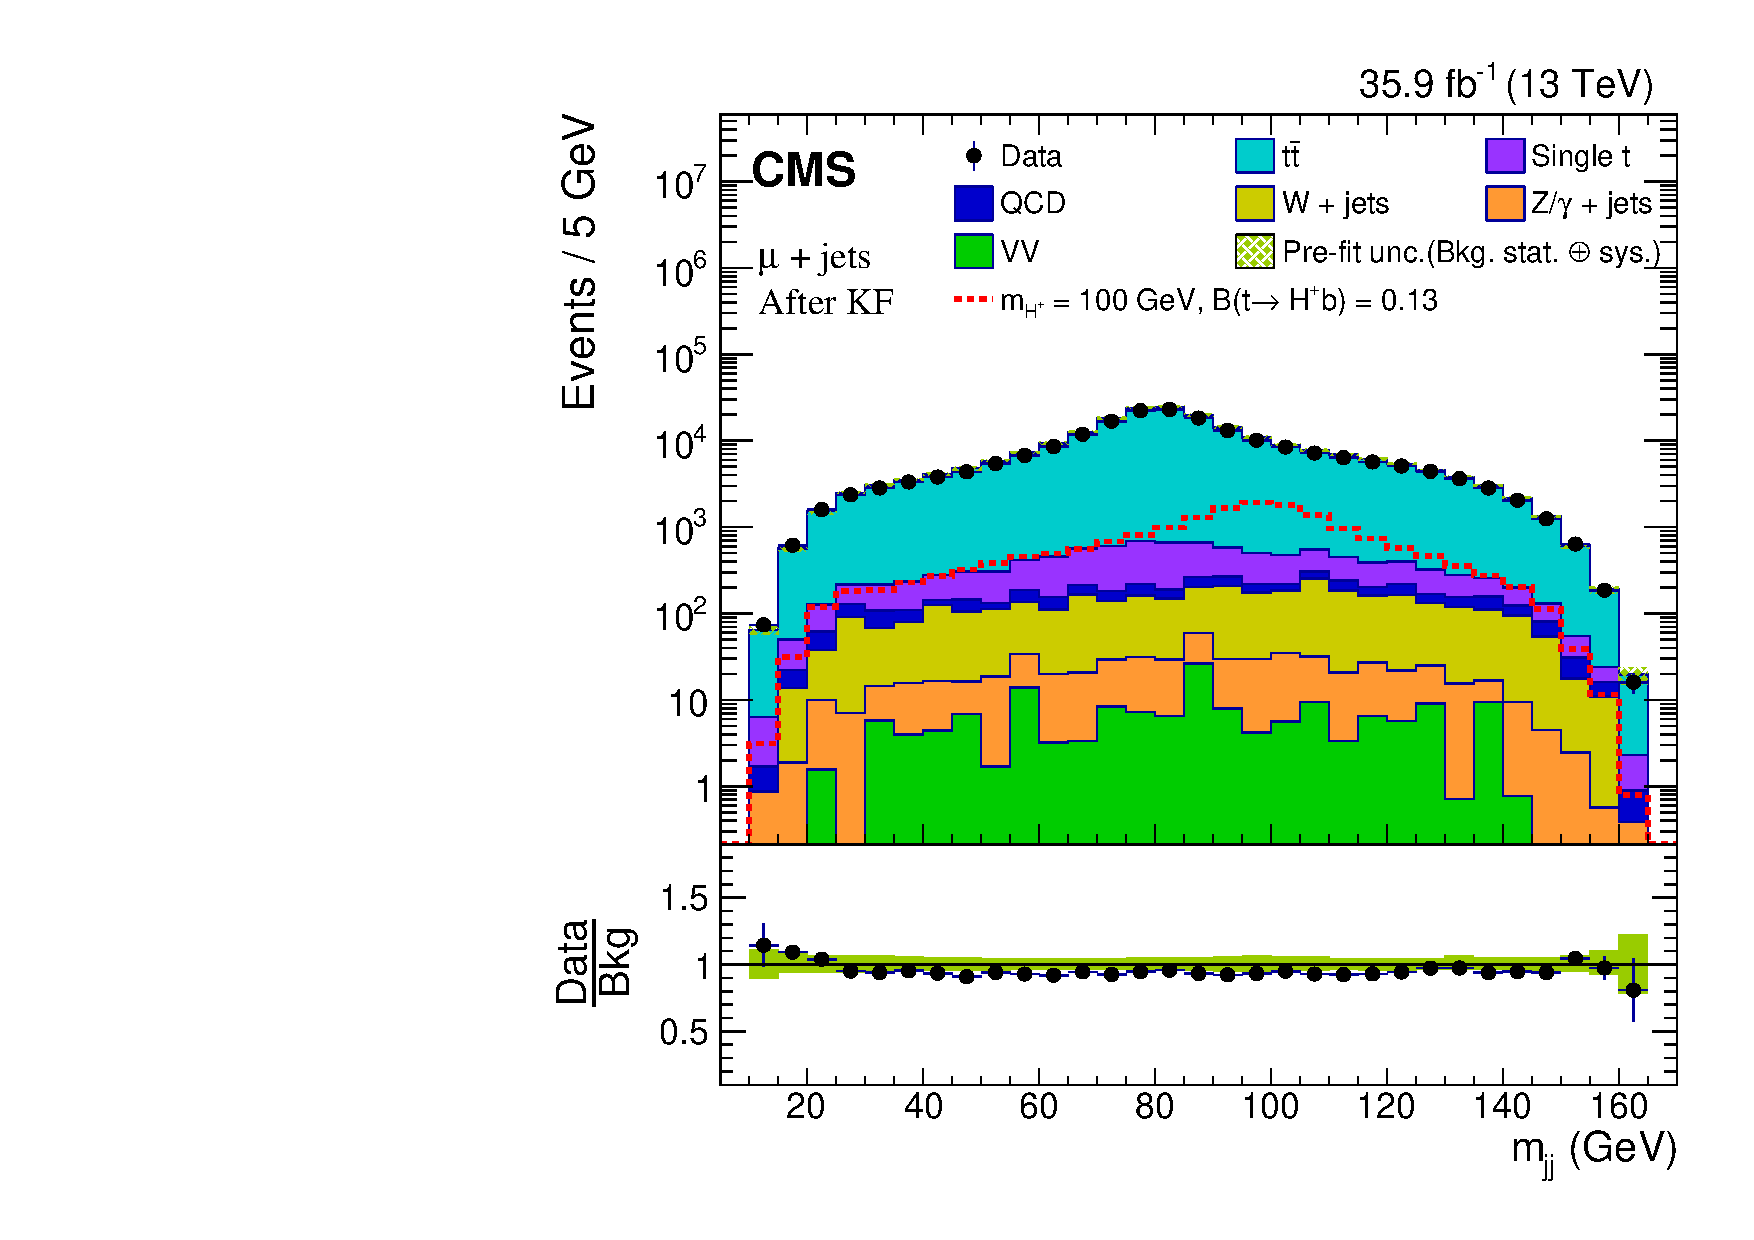
\includegraphics[width=0.49\linewidth]{Image/Muon/KinFit/mjj_kfit_muKinFit.pdf}}
    \subfigure[\mjj with kinematic fitted jets after KinFit selection \label{subfig:mjj_kfit_eleKinFit}]
    {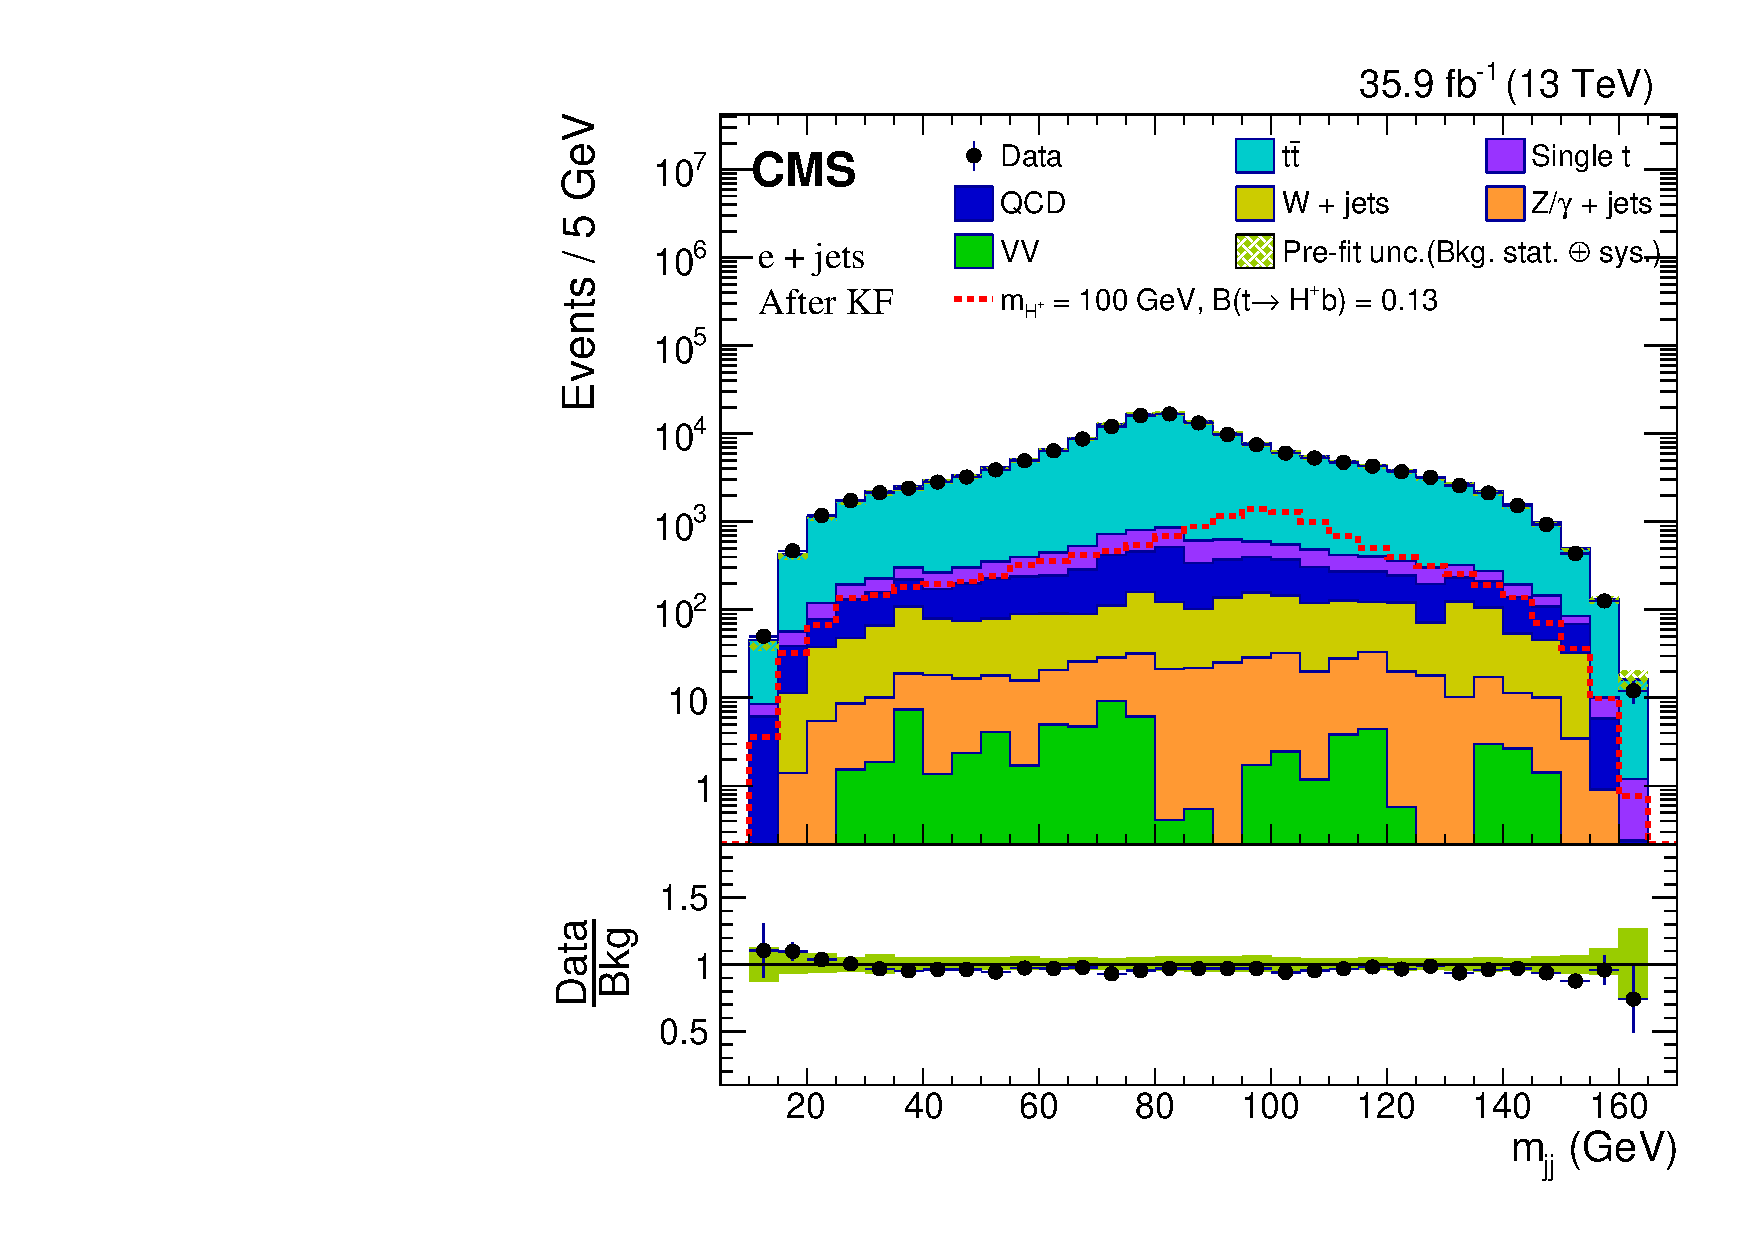
\includegraphics[width=0.49\linewidth]{Image/Electron/KinFit/mjj_kfit_eleKinFit.pdf}}
    \caption{\mjj distributions of two non-b, highest \pt-jets for the 
     \mujets and \ejets channel. The distributions of 
     Figure~\ref{subfig:mjj_muBTag} and \ref{subfig:mjj_eleBTag} are obtained 
     using reconstructed jets after applying b-tag scale factor as described 
     in Sec.~\ref{s:secEvtSel}. On the other hand, the distributions of 
     Figure~\ref{subfig:mjj_kfit_muKinFit} and \ref{subfig:mjj_kfit_eleKinFit} 
     are calculated using kinematic fitted jets after kinematic fit selection. 
     The mean of the invariant mass distribution from kinematic fitted jets 
     is closer to the W mass as compared to that of reconstructed jets.}
    \label{fig:mjjBTagKinFit}
\end{figure}

To select true semi-leptonic \ttbar events, a kinematic fit is performed on the 
reconstructed objects using the top kinematic fitter package~\cite{DHondt:2006iej}. 
The \verb|TopKinFitter| takes physics objects such as lepton, jets, \MET, and their 
resolutions as input, and gives improved four-vectors of lepton, jets, and neutrino with 
associated $\chi^2$ and probability of the fit as output. It constrains the reconstructed 
top-quark mass to its nominal value ($m_t = 172.5$ GeV). In the output, the 
\verb|TopKinFitter| gives only 4-jets (2 b-jets from leptonic and hadronic modes, and 2 
light-jets from hadronic mode), 1 lepton, and neutrino. It also separates jets coming from
leptonic and hadronic decay modes of \ttbar. The 2 light-jets coming from hadronic 
decay mode are further used for charm-tagging. A more detailed description of the 
kinematic fitting is given below.

\subsection{Input to the TopKinFitter}
\label{ss:inputKF} 
After applying identification and selection criteria on physics objects as described
in Section (\ref{s:secReco}), the event passed to the \verb|TopKinFitter| contains only one lepton, 
\MET and at least 4 jets. The b-discriminator value with the medium working point is also 
given as the input to the TopKinFitter to separate b-jet from light jets (more details in 
Section (\ref{ss:jetSepKF})). The constraints on the ttbar system along with the 
theoretical mass of the top-quark are also specified (more details in Section 
(\ref{ss:constraintKF})). All the constraints and invariant mass are parameterized in 
terms of $E_{T}$, $\eta$, and $\phi$ variables of the physics objects. The components of 
4-momentum vector in terms of these variables are given as
\begin{equation}
E = E_{T} \sin\theta, p_x = E_{T}\cos\phi, p_y = E_{T}\sin\phi, p_z = E_{T}\cot\theta,
\end{equation}
And the invariant mass of two particles, in the relativistic limit, is given by
\begin{equation}
	M_{inv} = \sqrt{2 E_{T1}E_{T2}\left(\cosh(\eta_1 - \eta_2) - \cos(\phi_1 - \phi2)\right)}
\end{equation}
Where $\eta = \ln\cot(\theta/2)$. The resolution of each physics object as a function of 
pt and eta, and the JER scale factors from different $\eta$ binning are also given in the 
input. Apart from the physics objects, various inputs related to the minimization of 
$\chi^2$ such as the maximum number of iterations, criteria on the convergence of the $\chi^2$
are also specified (more details in Section (\ref{ss:chi2KF})).

\subsection{Separation of jets}
\label{ss:jetSepKF} 
For the semileptonic decay mode of the ttbar, the first step is to separate 2 
b-jets from light-jets and the second step is to identify each b-jet from hadronic 
and leptonic modes.  All the jets are sorted in their \pt order and first 4 jets are
selected. To find out the two b-jets, a b-tag probability is calculated using 
following formula \cite{DHondt:2006iej}
\begin{equation}
	L_{b}(x) = \frac{PDF_b(x)}{\sum_{i=1}^5 PDF_i(x)}
\end{equation}
Where $PDFi(x)$ is the probability distribution function of b-tag discriminator value
(x) for flavour $i$. An event is selected if two jets have b-tag probability of more 
than 60\%. The jet-parton matching is also performed for each jet. For n number of 
jets, there are exactly n number of partons. The number of permutations in the 
jet-parton matching is given by
\begin{equation}
	N_{perm} = \frac{n!}{n-4)!}
\end{equation}
Therefore for 4 jets, there are 24 permutations. All the 24 permutations are shown 
in \cite{KinFitThesis} through diagrams. However, after identifying two b-jets, the number of 
permutations reduces to 12 as the two b-jets are interchangeable. For each 
jet-parton permutation, a $\chi^2$ is constructed, as described in Section 
(\ref{ss:chi2KF}), and the permutation with the lowest value of $\chi^2$ is
treated as the correct matching. Afterward, three jets (1 b-jet and 2 light-jets) 
have to be selected to form hadronic decaying top-quark. For this, several sensitive 
variables are used \cite{DHondt:2006iej} such as the angle between jets and lepton, 
angular separation between the generated and reconstructed jets, etc.

\subsection{Kinematic constraints}
\label{ss:constraintKF} 
The semileptonic decay mode of the \ttbar has 4 jets, 1 lepton and the neutrino in the final
state.The x and y-component of the neutrino are taken from the \MET, as the 
missing transverse energy is attributed to the neutrino. And the z-component of the 
neutrino, $p^v_z$, is determined from the fit. The following kinematic constraints are 
imposed on the semileptonic \ttbar system
\begin{subequations}
\begin{eqnarray}
	m_{inv}(b^{had}q\bar{q}) = m_{t} = 172.5 ~GeV \label{eq:constraintKF1}\\
	m_{inv}(b^{lep}l\nu_l)   = m_{\bar{t}} = 172.5 ~GeV \label{eq:constraintKF2}
\end{eqnarray}
\label{eq:constraintKF}
\end{subequations}
After the fit, the $p^v_z$ is determined from the Equation (\ref{eq:constraintKF2}). 
For every event, a $\chi^2$ is constructed as discussed in Section (\ref{ss:chi2KF}).
The $\chi^2$ is minimized by varying Pt, $\eta$, and $\phi$ of each object within
their resolution. Those values of Pt, $\eta$, and $\phi$ variables are finally selected 
which minimises the $\chi^2$ and at the same time satisfies the Equation (\ref{eq:constraintKF}).

\subsection{Chi-square of the fit}
\label{ss:chi2KF} 
For every selected event, a $\chi^2$ is constructed as given by [$AN2012\_477$]
\begin{equation}
	\chi^2 = \left(\frac{m_t - 172.5}{\sigma_{m_{t}}}\right)^2 + 
	\left(\frac{m_{\bar{t}} - 172.5}{\sigma_{m_{\bar{t}}}}\right)^2+
	\sum_{i}\left(\frac{p_i^{fit, lep} - p_i^{lep}}{\sigma_{p^{lep}_i}}\right)^2+
	\sum_{j}\sum_{i}\left(\frac{p_i^{fit, jet_j} - 
	p_i^{jet_j}}{\sigma_{p^{jet_j}_i}}\right)^2
\label{eq:chi2KF}
\end{equation}
where $\sigma_{m_{t}}$ is the resolution of the mass of the top-quark and $\sigma_{p_{i}}$ 
is the momentum resolution of three component ($i= 1, 2, 3$) of the lepton and jets.
The $p^{fit}$ is the fitted momentum of lepton and jets. The $\chi^2$, given in Equation
(\ref{eq:chi2KF}) is minimized using the Lagrangian multipliers under the constraints 
given in Equation (\ref{eq:constraintKF}).

A detailed mathematical description for the minimization of the $\chi^2$ is
given in \cite{DHondt:2006iej}. The $\chi^2$ is minimized iteratively wherein each step 
the 4 components of the momentum vector of each object are varied
within their resolution and a $\chi^2$ and the constraint is calculated. 
The object resolutions used in the kinematic fitting are conservative, 
derived from from 8 \TeV analysis. The fit is declared to be converged 
if the following condition is satisfied
\begin{subequations}
\begin{eqnarray}
	\frac{\chi^2 (n-1) - \chi^2 (n)}{ndf} < \epsilon_{\chi}\\ 
	m_{inv}(b^{had}q\bar{q}) - 172.5 < \epsilon_{c}\\
        m_{inv}(b^{lep}l\nu_l) - 172.5 < \epsilon_{c}
\end{eqnarray}
\end{subequations}
where $\epsilon_{\chi} = 5\times 10^{-05}$, $\epsilon_{c} = 0.0001$, and $ndf$
is the number of degrees of freedom which is equal to 1 as we have two 
constraints and one free parameter ($p_z^\nu$). The total number of iterations ($n$)
is 500.

\subsection{Output of the KinFit}
\label{ss:outputKF} 
For every event, the \verb|TopKinFitter| gives the status of fit which is 0 if 
the fit converged and 1 if it did not, $\chi^2$ of the fit, probability ($P_{\chi}$) 
of the goodness-of-fit of $\chi^2$, and the 4 momentum vector of physics objects such
as jets, lepton and a neutrino. The $\chi^2$ and $P_{\chi}$ are related by the 
following equation
\begin{equation}
	P_{\chi} = \exp(\frac{-\chi^2}{2})
\end{equation}
The fit also separates jets from hadronic and leptonic decay mode of \ttbar, 
that is, it gives hadronic 1 b-jet, 1-leptonic b-jet, and 2 light jets from hadronic
decay separately. The c-tagging criteria are applied further on the 2 light jets as 
discussed in Section \ref{s:cTag}. The \mjj distribution of the light jets is used in 
further analysis.

\subsection{Selection and Performance}
\label{ss:selKF} 
Due to wrong jet combinatorics, the fit does not converge for every event. Only
those events are selected for which the fit converges. The efficiency of fit
convergence is 73\% for MC \ttbar sample and 71\% for data for both channels.
Further, the angular separation between reconstructed and kinematic fitted 
lepton and jets are required to be less than 0.2 to make sure that they are in the same
direction. The same $\Delta R$ cut is applied on reconstructed jets and kinematic
fitted jets. Also, the \pt cut on kinematic fitted lepton and jets are required to
be the same as that on the reconstructed jets and lepton. After applying these additional 
cut on $\Delta R$ and \pt, the kinematic fit efficiency reduces to 47\% for \ttbar 
and 44\% for data for both channels. The \mjj distribution from the two 
light jets after KinFit selection is shown in (~\ref{subfig:mjj_kfit_muKinFit})  
and (\ref{subfig:mjj_kfit_eleKinFit}) for both channels. The mean value of the 
\mjj distribution is 84 GeV for both channels.
%The KinFit efficiency at 8 TeV was also 47\% for \ttbar sample. The 
%distribution of $\chi^2$ and $P_{\chi^2}$ after the KinFit
%selections are shown in Figure (). Various cuts on $\chi^2$ and $P_{\chi}$ were
%tried at 8 TeV. However, none of them improved the expected limits and finally, no cut
%on these was applied. At 13 TeV also, we don't apply any cut on these. 

The KinFit is performed after applying jet energy corrections such as JES and JER.
For up and down systematics of JES and JER, the KinFit is performed separately 
on every event after correcting jet \pt using the corresponding scale factors.
The output of the KinFit for each systematic is stored in a different collection
using the \verb|EDProducer|. The kinematic fitting is a time-consuming process 
which takes, on average 0.002 seconds per event for \ttbar process. Therefore, 
performing all (nominal, \verb|JESup|, \verb|JESdown|, \verb|JERup|, and 
\verb|JERdown|) the kinematic fitting takes a reasonable amount of time.
